\documentclass{article}
\usepackage[a4paper,margin=2cm]{geometry}
\usepackage[ngerman]{babel}
\usepackage{graphicx}
\usepackage{booktabs}
%\usepackage{siunitx}
\usepackage{pgfplots}
\usepackage{tikz}
\usepackage{pgfplots}
\usepackage{multicol}
\usepackage{mathrsfs}

\pgfplotsset{width=10cm,compat=1.18}
\usetikzlibrary{arrows}
\setlength{\parindent}{0pt}


\title{Kondensatoren}
\author{Daniel Renschler}
\date{28. M\"arz 2023}


\begin{document}
\maketitle


%%%%%%%%    ABSTRACT ANFANG     %%%%%%%%
%\begin{center}
%\begin{minipage}{0.9\textwidth}
%\begin{center}
%\rule{1\textwidth}{1pt}
%\begin{abstract}
  %ABSTRACT
%\end{abstract}
%\end{center}
%\vspace{0.1cm}
%\end{minipage}
%\end{center}
%\vspace{-.5cm}
%\hspace{1.5cm}\textit{Schlüsselwörter: }%\textsf{}
%\vspace{-.2cm}
%\begin{center}
%\rule{.9\textwidth}{1pt}
%\end{center}
%%%%%%%%    Ziel des Versuchs   %%%%%%%%


\begin{multicols}{2}
\section{Ziel des Versuchs}
Ziel des Versuchs ist die Kondensatoren zu verstehen und wie sie funktionieren.


%%%%%%%%    Thematischer Kontext und behauptung %%%%%%%%%
\section{Thematischer Kontext und ggf. die zu überprüfende Behauptung}
Im thematischen Kontext der Elektrotechnik spielt der Lade- und Entladevorgang
von Kondensatoren eine wichtige Rolle. Kondensatoren werden in vielen
elektronischen Anwendungen eingesetzt, beispielsweise in Schaltungen oder als
Energiespeicher. Daher ist es von Bedeutung, die Eigenschaften von
Kondensatoren und ihre Reaktion auf verschiedene Parameter wie Kapazität und
Widerstand im Stromkreis zu verstehen.

Die zu überprüfende Behauptung in diesem Versuch war, dass die Kapazität und
der Widerstand im Stromkreis signifikante Auswirkungen auf den Lade- und
Entladevorgang eines Kondensators haben. Durch die Durchführung von Messungen
unter Verwendung verschiedener Kapazitäten und Widerstände sollte diese
Behauptung überprüft und deren Einfluss auf den Lade- und Entladevorgang von
Kondensatoren untersucht werden.

%%%%%%%%    Ort/namen informationen zur Durchführung %%%%%%%%
\section{Ort und Zeit der Durchführung, Namen der Experimentator:innen}
Der Versuch wurde am 28.03.2023 an der Rolf-Benz-Schule in Nagold im Raum 349
von Daniel Renschler durchgeführt. 


%%%%%%%%    Beschreibung des Veruschs mit Versuchsaufbau    %%%%%%%%
\end{multicols}
\section{Beschreibung und ggf. Versuchsaufbau}

\begin{figure}[!htb]
    \centering
    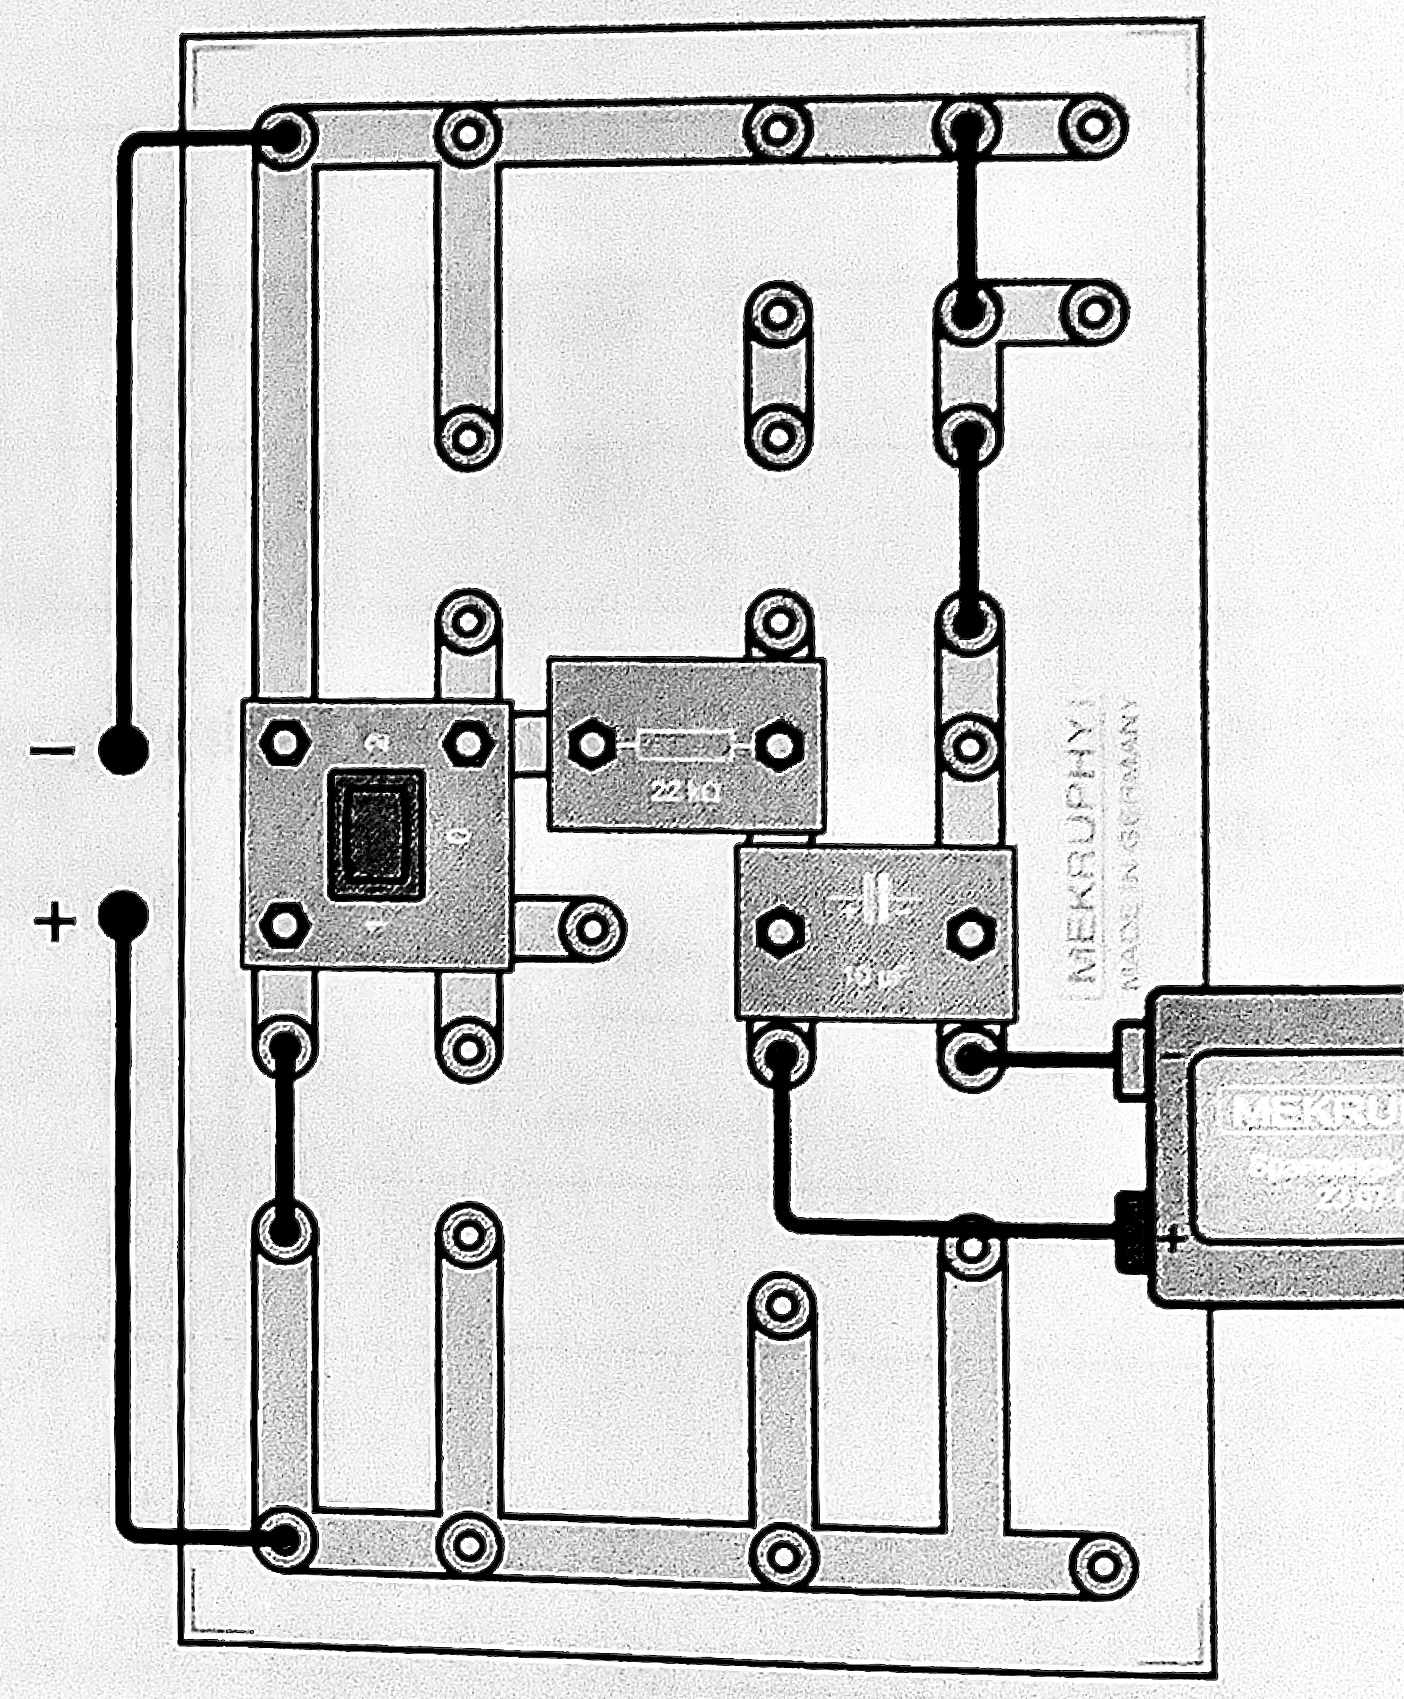
\includegraphics[width=.2\textwidth]{aufbau.jpg}
    \caption{Vorgegebener Versuchsaufbau (E5 - 11)}
    \label{fig:versuchsaufbau}
\end{figure}


%%%%%%%%    Beschreibung der Versuchsdurchführung   %%%%%%%%
\section{Beschreibung der Versuchsdurchführung}
Für den Versuch hat man den Versuch aufgebaut wie vorgegeben in Abbildung
\ref{fig:versuchsaufbau}, dann muss man das MGA richtig einstellen sowie
vorgegeben.




%%%%%%%%    Messergebnisse mit Veranschaulichung   %%%%%%%%
\section{Messergebnisse und ggf. grafische Veranschaulichung}

Für die Messung wurden die Ladezeit, Entladezeit und die maximale Spannung
während des Lade- und Entladevorgangs aufgenommen. Die Ergebnisse sind in der
folgenden Tabelle dargestellt:

\begin{table}[!htb]
\centering
\caption{Ergebnisse des Versuchs zum Laden und Entladen eines Kondensators}
\label{tab:KondensatorErgebnisse}
\begin{tabular}{@{}llllll@{}}
\toprule
Kapazität & Widerstand & Ladezeit & Entladezeit & Max. Spannung\\
\midrule
10$\mu$F & 22k$\Omega$ & 1,04 s & 1,2 s & 4,95 V &\\
4,7$\mu$F & 22k$\Omega$ & 0,7653 s & 0,79 s & 5,055 V\\
4,7$\mu$F & 10k$\Omega$ & 0,4082 s & 0,382 s & 4,977 V\\
\bottomrule
\end{tabular}
\end{table}


\begin{multicols}{2}
%%%%%%%%%%% Fehlerbetrachtung %%%%%%%%%%%
%\section{Fehlerbetrachtung}



%%%%%%%%%%% Schlussfolgerung %%%%%%%%%%%
\section{Interpretation und Schlussfolgerung}
Die Ergebnisse zeigen, dass die Kapazität und der Widerstand des Kondensators
einen signifikanten Einfluss auf den Lade- und Entladevorgang haben. Eine
höhere Kapazität des Kondensators führt zu längeren Lade- und Entladezeiten, da
mehr Ladung aufgenommen und freigesetzt werden muss. Eine höhere Kapazität
führt jedoch auch zu einer höheren maximalen Spannung während des Ladevorgangs,
da mehr Ladung gespeichert werden kann.

Ein höherer Widerstand im Stromkreis führt ebenfalls zu längeren Lade- und
Entladezeiten, da der Stromfluss durch den Widerstand begrenzt wird. Dies führt
zu einer niedrigeren maximalen Spannung während des Ladevorgangs. Eine
niedrigere Widerstandswertung ermöglicht eine schnellere Ladung und Entladung
und eine höhere maximale Spannung während des Ladevorgangs.

\end{multicols}
\end{document}
